%%%%%%%%%%%%%%%%%%%%%%%%%%%%%%%%%%%%%%%%%
% Beamer Presentation
% LaTeX Template
% Version 1.0 (10/11/12)
%
% This template has been downloaded from:
% http://www.LaTeXTemplates.com
%
% License:
% CC BY-NC-SA 3.0 (http://creativecommons.org/licenses/by-nc-sa/3.0/)
%
%%%%%%%%%%%%%%%%%%%%%%%%%%%%%%%%%%%%%%%%%

%----------------------------------------------------------------------------------------
%	PACKAGES AND THEMES
%----------------------------------------------------------------------------------------

\documentclass{beamer}

\mode<presentation> {

% The Beamer class comes with a number of default slide themes
% which change the colors and layouts of slides. Below this is a list
% of all the themes, uncomment each in turn to see what they look like.

%\usetheme{default}
%\usetheme{AnnArbor}
%\usetheme{Antibes}
%\usetheme{Bergen}
%\usetheme{Berkeley}
%\usetheme{Berlin}
%\usetheme{Boadilla}
%\usetheme{CambridgeUS}
%\usetheme{Copenhagen}
\usetheme{Darmstadt}
%\usetheme{Dresden}
%\usetheme{Frankfurt}
%\usetheme{Goettingen}
%\usetheme{Hannover}
%\usetheme{Ilmenau}
%\usetheme{JuanLesPins}
%\usetheme{Luebeck}
%\usetheme{Madrid}
%*\usetheme{Malmoe}
%\usetheme{Marburg}
%\usetheme{Montpellier}
%\usetheme{PaloAlto}
%\usetheme{Pittsburgh}
%\usetheme{Rochester}
%\usetheme{Singapore}
%\usetheme{Szeged}
%\usetheme{Warsaw}

% As well as themes, the Beamer class has a number of color themes
% for any slide theme. Uncomment each of these in turn to see how it
% changes the colors of your current slide theme.

%\usecolortheme{albatross}
%\usecolortheme{beaver}
%\usecolortheme{beetle}
%\usecolortheme{crane}
%\usecolortheme{dolphin}
%\usecolortheme{dove}
%\usecolortheme{fly}
%\usecolortheme{lily}
\usecolortheme{orchid}
%\usecolortheme{rose}
%\usecolortheme{seagull}
%\usecolortheme{seahorse}
%\usecolortheme{whale}
%\usecolortheme{wolverine}

%\setbeamertemplate{footline} % To remove the footer line in all slides uncomment this line
%\setbeamertemplate{footline}[page number] % To replace the footer line in all slides with a simple slide count uncomment this line

%\setbeamertemplate{navigation symbols}{} % To remove the navigation symbols from the bottom of all slides uncomment this line
}


\usepackage{graphicx} % Allows including images
\usepackage{booktabs} % Allows the use of \toprule, \midrule and \bottomrule in tables
\usepackage{xspace}
\usepackage{caption}
\usepackage{subfigure}
\usepackage[english,brazil]{babel}
\usepackage[utf8]{inputenc}

%Renomeia o nome padrao das figuras.
\renewcommand{\figurename}{Figura}
\renewcommand{\tablename}{Tabela}
%----------------------------------------------------------------------------------------
%	TITLE PAGE
%----------------------------------------------------------------------------------------

\title[Computação Gráfica]{Transformações 3D} % The short title appears at the bottom of every slide, the full title is only on the title page

\author{Uéliton Freitas} % Your name
\institute[UFMS] % Your institution as it will appear on the bottom of every slide, may be shorthand to save space
{
Universidade Católica Don Bosco - UCDB \\ % Your institution for the title page
\medskip
\textit{freitas.ueliton@gmail.com} % Your email address
}
\date{\today} % Date, can be changed to a custom date


\begin{document}

\begin{frame}
\titlepage % Print the title page as the first slide
\end{frame}

\begin{frame}
\frametitle{Sumário} % Table of contents slide, comment this block out to remove it
\tableofcontents % Throughout your presentation, if you choose to use \section{} and \subsection{} commands, these will automatically be printed on this slide as an overview of your presentation
\end{frame}




%----------------------------------------------------------------------------------------
%	PRESENTATION SLIDES
%----------------------------------------------------------------------------------------

%------------------------------------------------
\section{Introdução} 
%------------------------------------------------

%\section{Speeded-Up Robust Features - SURF} % A subsection can be created just before a set of slides with a common theme to further break down your presentation into chunks
%\section{Baf Of Features and Colors}

%\section{Refer\^encias}
%%%%%%%%%%%%%%%%%%%%%%%%%%%%%%%%%%%%%%%%%%%%%%%%%%%%%%%%%%%%%%%%%%%%%%%%%%%%%%%%%%%%%%%%%%
\begin{frame}
\frametitle{Introdução}


	\begin{block}{Transformações 3D}
		\begin{itemize}
			\item<1-> Transformações 3D são extensões das transformações 2D.
			\item<2-> A translação e escala são simples adaptações.
			\item<3-> A rotação é mais complexa.
				\begin{itemize}
					\item Pode-se efetuar a rotação em qualquer eixo espacial. Diferente da rotação 2D que é feita em torno do eixo $x,y$.
				\end{itemize}
			\item<4-> As posições 3D são expressadas por coordenadas homogêneas por meio de matrizes com 4 linhas e colunas, ou seja, as matrizes 3D são $4x4$.
		\end{itemize}
	\end{block}
	
\end{frame}


%%%%%%%%%%%%%%%%%%%%%%%%%%%%%%%%%%%%%%%%%%%%%%%%%%%%%%%%%%%%%%%%%%%%%%%%%%%%%%%%%%%%%%%%%%
\section{Transformações Básicas}
\subsection{Translação}
\begin{frame}
\frametitle{Translação}


	\begin{block}{Translação 3D}
		\begin{itemize}
			\item Um objeto é deslocado adicionando-se um deslocamento a cada uma das direções cartesianas.
			\begin{eqnarray*}
				x' = x + \Delta x \\
				y' = y + \Delta y \\
				z' = z + \Delta z \\
			\end{eqnarray*}
		\end{itemize}
	\end{block}
	
\end{frame}

%%%%%%%%%%%%%%%%%%%%%%%%%%%%%%%%%%%%%%%%%%%%%%%%%%%%%%%%%%%%%%%%%%%%%%%%%%%%%%%%%%%%%%%%%%
\begin{frame}
\frametitle{Translação}

	\begin{block}{Representação Matricial da Translação 3D}
		
			\begin{eqnarray*}
				P' = T(\Delta x,\Delta y,\Delta z) \cdot P\\
				\begin{bmatrix}
					x'	\\
					y'	\\
					z'	\\
					1
				\end{bmatrix}								
				= \begin{bmatrix}
					1	&	0	&	0	&	\Delta x	\\
					0	&	1	&	0	&	\Delta y	\\
					0	&	0	& 	1	&	\Delta z	\\
					0	&	0	&	0	&	1		\\
				\end{bmatrix}
				\cdot \begin{bmatrix}
					x	\\
					y	\\
					z	\\
					1
				\end{bmatrix}
			\end{eqnarray*}
	
	\end{block}

	
	
\end{frame}

%%%%%%%%%%%%%%%%%%%%%%%%%%%%%%%%%%%%%%%%%%%%%%%%%%%%%%%%%%%%%%%%%%%%%%%%%%%%%%%%%%%%%%%%%%
\begin{frame}
\frametitle{Translação}

	\begin{figure}[!h]
			\begin{center}
			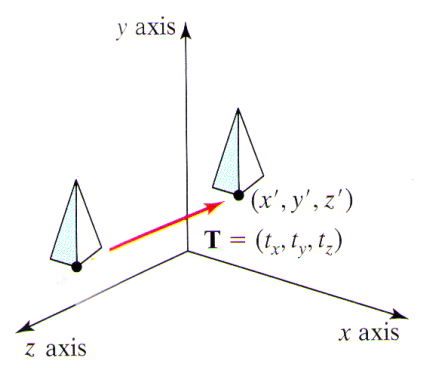
\includegraphics[width=0.5\textwidth]{Figures/translacao3D}
			\end{center}
	\end{figure}	
\end{frame}


%%%%%%%%%%%%%%%%%%%%%%%%%%%%%%%%%%%%%%%%%%%%%%%%%%%%%%%%%%%%%%%%%%%%%%%%%%%%%%%%%%%%%%%%%%
\begin{frame}
\frametitle{Translação Inversa}

	\begin{block}{Representação Matricial da Translação 3D Inversa}
		
			\begin{eqnarray*}
				T^{-1}(\Delta x,\Delta y,\Delta z) =  T(- \Delta x,- \Delta y, -\Delta z)\\
			T^{-1}(\Delta x,\Delta y,\Delta z) = \begin{bmatrix}
					1	&	0	&	0	&	-\Delta x	\\
					0	&	1	&	0	&	-\Delta y	\\
					0	&	0	& 	1	&	-\Delta z	\\
					0	&	0	&	0	&	1		\\
				\end{bmatrix}
			\end{eqnarray*}
	\end{block}
\end{frame}

%%%%%%%%%%%%%%%%%%%%%%%%%%%%%%%%%%%%%%%%%%%%%%%%%%%%%%%%%%%%%%%%%%%%%%%%%%%%%%%%%%%%%%%%%%
\subsection{Escala 3D}
\begin{frame}
\frametitle{Escala}

	\begin{block}{Escala 3D}
		\begin{itemize}
			\item A escala 3D é uma simples extensão da escala 2D.
			\begin{eqnarray*}
				s_x > 0, s_y > 0,s_z > 0 \\
				x' = x \cdot s_x \\
				y' = y \cdot s_y \\
				z' = z \cdot s_z \\
			\end{eqnarray*}
		\end{itemize}
	\end{block}
\end{frame}


%%%%%%%%%%%%%%%%%%%%%%%%%%%%%%%%%%%%%%%%%%%%%%%%%%%%%%%%%%%%%%%%%%%%%%%%%%%%%%%%%%%%%%%%%%
\begin{frame}
\frametitle{Escala}

	\begin{block}{Representação Matricial da Escala 3D}
		\begin{itemize}
			\item A escala 3D é uma simples extensão da escala 2D.
			\begin{eqnarray*}
				P' = S(s_x,s_y,s_z) \cdot P\\
				\begin{bmatrix}
					x'	\\
					y'	\\
					z'	\\
					1
				\end{bmatrix}								
				= \begin{bmatrix}
					s_x	&	0	&	0	&	0	\\
					0	&	s_y	&	0	&	0	\\
					0	&	0	& 	s_z	&	0	\\
					0	&	0	&	0	&	1	\\
				\end{bmatrix}
				\cdot \begin{bmatrix}
					x	\\
					y	\\
					z	\\
					1
				\end{bmatrix}
			\end{eqnarray*}
		\end{itemize}
	\end{block}
\end{frame}


%%%%%%%%%%%%%%%%%%%%%%%%%%%%%%%%%%%%%%%%%%%%%%%%%%%%%%%%%%%%%%%%%%%%%%%%%%%%%%%%%%%%%%%%%%
\begin{frame}
\frametitle{Translação}

	\begin{block}{Escala 3D}
		\begin{itemize}
			\item Com $s_x > 1$ e $s_y > 1$
				\begin{itemize}
					\item O objeto se afasta da origem.
				\end{itemize}
				
			\item Com $ 0 <s_x < 1$ e $ 0 < s_y < 1$
				\begin{itemize}
					\item O objeto se aproxima da origem.
				\end{itemize}
		\end{itemize}
	\end{block}


	\begin{figure}[!h]
			\begin{center}
			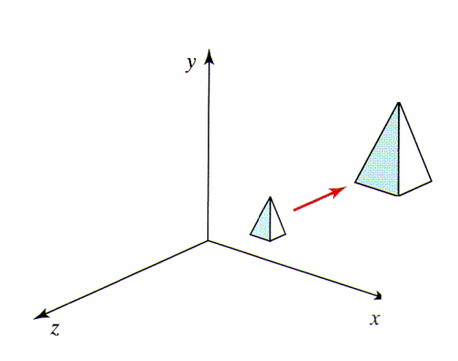
\includegraphics[width=0.5\textwidth]{Figures/Escala3D}
			\end{center}
	\end{figure}	
\end{frame}

%%%%%%%%%%%%%%%%%%%%%%%%%%%%%%%%%%%%%%%%%%%%%%%%%%%%%%%%%%%%%%%%%%%%%%%%%%%%%%%%%%%%%%%%%%
\begin{frame}
\frametitle{Translação}

	\begin{block}{Escala 3D - Ponto Fixo}
		\begin{itemize}
			\item Para resolver o problema do deslocamento:
				\begin{itemize}
					\item Translada-se o ponto fixo do objeto para a origem.
					\item Efeuta-se a escala.
					\item Translada-se o ponto fixo para a posição original.\\
					$P' =T(\Delta x_f, \Delta y_f, \Delta z_f) \cdot S(s_x,s_y,s_z) \cdot T(- \Delta x_f, - \Delta y_f, - \Delta z_f)$
					\begin{eqnarray*}
						\begin{bmatrix}
							x'	\\
							y'	\\
							z'	\\
							1
						\end{bmatrix}								
				= \begin{bmatrix}
					s_x	&	0	&	0	&	(1-s_x)x_f	\\
					0	&	s_y	&	0	&	(1-s_y)y_f	\\
					0	&	0	& 	s_z	&	(1-s_z)z_f	\\
					0	&	0	&	0	&	1	\\
				\end{bmatrix}
				\cdot \begin{bmatrix}
					x	\\
					y	\\
					z	\\
					1
				\end{bmatrix}
			\end{eqnarray*}
			\end{itemize}
		\end{itemize}
	\end{block}
\end{frame}


%%%%%%%%%%%%%%%%%%%%%%%%%%%%%%%%%%%%%%%%%%%%%%%%%%%%%%%%%%%%%%%%%%%%%%%%%%%%%%%%%%%%%%%%%%
\begin{frame}
\frametitle{Escala Inversa}

	\begin{block}{Escala Inversa 3D}
		\begin{itemize}
			\item A matriz da escala inversa é obtida trocando os valores das escalas por seus valores inversos.
			\begin{eqnarray*}
				T^{-1}(s_x,s_y,s_z) = \begin{bmatrix}
					\frac{1}{s_x}	&	0	&	0	&	(1-\frac{1}{s_x})x_f	\\
					0	&	\frac{1}{s_y}	&	0	&	(1-\frac{1}{s_y})y_f	\\
					0	&	0	& 	\frac{1}{s_z}	&	(1-\frac{1}{s_z})z_f	\\
					0	&	0	&	0	&	1	\\
				\end{bmatrix}
			\end{eqnarray*}
		\end{itemize}
	\end{block}
\end{frame}


%%%%%%%%%%%%%%%%%%%%%%%%%%%%%%%%%%%%%%%%%%%%%%%%%%%%%%%%%%%%%%%%%%%%%%%%%%%%%%%%%%%%%%%%%%
\subsection{Rotação 3D}
\begin{frame}
\frametitle{Rotação 3D}

	\begin{block}{Rotação 3D}
		\begin{itemize}
			\item Pode-se rotacionar um objeto em qualquer eixo no espaço 3D.
			\item Contudo, é mais fácil fazer a rotação sobre os eixos cartesianos.
				\begin{itemize}
					\item É possível combinar qualquer rotação em torno dos eixos cartesianos para obter rotações em qualquer eixo no espaço.
				\end{itemize}
			\item Ângulos positivos rotacionam o objeto no sentido anti-horário.
		\end{itemize}
	\end{block}
\end{frame}

%%%%%%%%%%%%%%%%%%%%%%%%%%%%%%%%%%%%%%%%%%%%%%%%%%%%%%%%%%%%%%%%%%%%%%%%%%%%%%%%%%%%%%%%%%
\begin{frame}
\frametitle{Orientação da Rotação 3D}

	\begin{figure}[!h]
			\begin{center}
			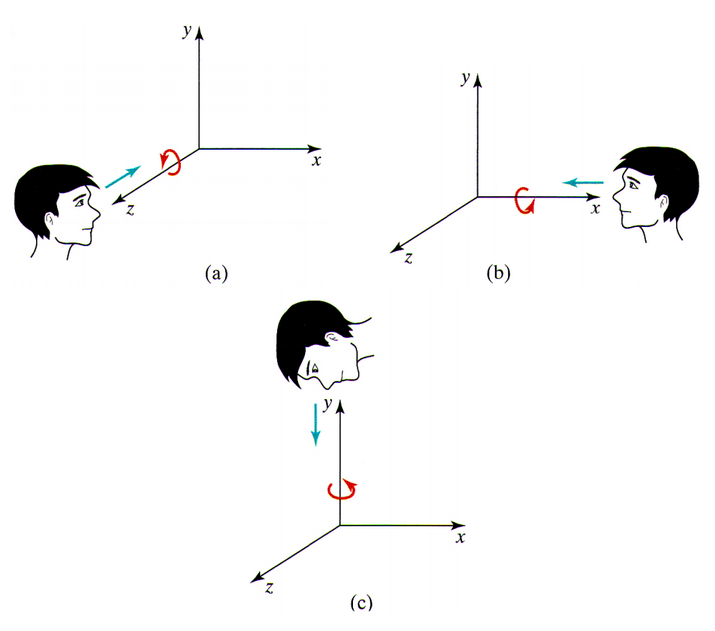
\includegraphics[width=0.7\textwidth]{Figures/OriRotacao}
			\end{center}
	\end{figure}
	
\end{frame}


%%%%%%%%%%%%%%%%%%%%%%%%%%%%%%%%%%%%%%%%%%%%%%%%%%%%%%%%%%%%%%%%%%%%%%%%%%%%%%%%%%%%%%%%%%
\begin{frame}
\frametitle{Orientação da Rotação 3D}

	\begin{block}{Rotação 3D}
		\begin{itemize}
			\item A rotação 3D pode ser facilmente estendida da rotação 2D.
			\begin{eqnarray*}
				x' = x \cdot cos \theta - y \cdot sen \theta \\
				y' = x \cdot sen \theta - y \cdot cos \theta \\
				z' = z
			\end{eqnarray*}
		\end{itemize}
	\end{block}
	
	\begin{block}{Rotação 3D na Representação Matricial}
		\begin{itemize}
			\item A rotação 3D pode ser facilmente estendida da rotação 2D.
			\begin{eqnarray*}
				\textbf{P}' = \textbf{R}(\theta) \cdot \textbf{P}\\
				\begin{bmatrix}
					x'	\\
					y'	\\
					z'	\\
					1
				\end{bmatrix}
				= \begin{bmatrix}
					cos \theta	& -sen \theta	& 0 & 0 \\
					sen \theta	& cos \theta		& 0 & 0 \\
					0			& 0				& 1 & 0 \\
					0			& 0				& 0	& 1
				\end{bmatrix}
				\cdot \begin{bmatrix}
					x	\\
					y	\\
					z	\\
					1
				\end{bmatrix}
			\end{eqnarray*}
		\end{itemize}
	\end{block}
	
\end{frame}

%%%%%%%%%%%%%%%%%%%%%%%%%%%%%%%%%%%%%%%%%%%%%%%%%%%%%%%%%%%%%%%%%%%%%%%%%%%%%%%%%%%%%%%%%%
\begin{frame}
\frametitle{Rotação no eixo $z$}

	\begin{figure}[!h]
			\begin{center}
			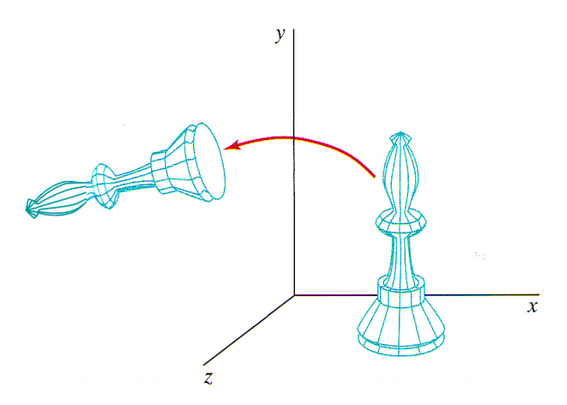
\includegraphics[width=0.7\textwidth]{Figures/Rz}
			\end{center}
	\end{figure}
	
\end{frame}


%%%%%%%%%%%%%%%%%%%%%%%%%%%%%%%%%%%%%%%%%%%%%%%%%%%%%%%%%%%%%%%%%%%%%%%%%%%%%%%%%%%%%%%%%%
\begin{frame}
\frametitle{Rotação 3D}

	\begin{block}{Rotação 3D}
		\begin{itemize}
			\item A rotação entre os eixos podem ser feitas por meio de uma permutação cíclica das coordenadas $x,y$ e $z$.\\
			$x \to y \to z \to x$
		\end{itemize}
	\end{block}

	\begin{figure}[!h]
			\begin{center}
			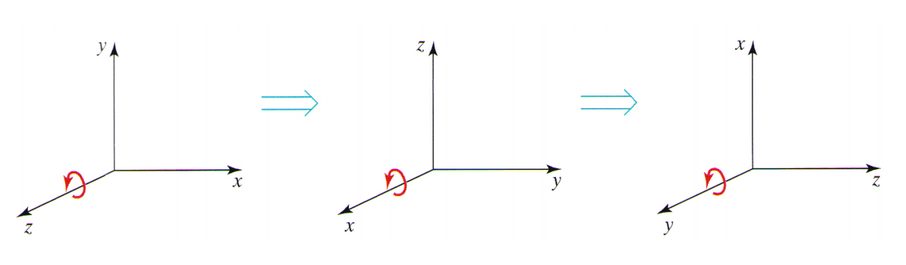
\includegraphics[width=0.9\textwidth]{Figures/Rcirc}
			\end{center}
	\end{figure}
	
\end{frame}

%%%%%%%%%%%%%%%%%%%%%%%%%%%%%%%%%%%%%%%%%%%%%%%%%%%%%%%%%%%%%%%%%%%%%%%%%%%%%%%%%%%%%%%%%%
\begin{frame}
\frametitle{Rotação 3D}

	\begin{block}{Rotação 3D no eixo $x$}
		\begin{itemize}
			\item Levando em consideração a permutação citada, a rotação no eixo $x$ é composta da seguinte equação:\\
			\begin{eqnarray*}
				\begin{bmatrix}
					x' \\
					y' \\
					z' \\
					1
				\end{bmatrix} = 
				\begin{bmatrix}
					1			& 0				& 0 & 0 \\
					cos \theta	& -sen \theta	& 0 & 0 \\
					sen \theta	& cos \theta		& 0 & 0 \\
					0			& 0				& 0	& 1
				\end{bmatrix}
				\cdot \begin{bmatrix}
					x \\
					y \\
					z \\
					1
				\end{bmatrix}
			\end{eqnarray*}
		\end{itemize}
	\end{block}
	
\end{frame}

%%%%%%%%%%%%%%%%%%%%%%%%%%%%%%%%%%%%%%%%%%%%%%%%%%%%%%%%%%%%%%%%%%%%%%%%%%%%%%%%%%%%%%%%%%
\begin{frame}
\frametitle{Rotação 3D}


	\begin{figure}[!h]
			\begin{center}
			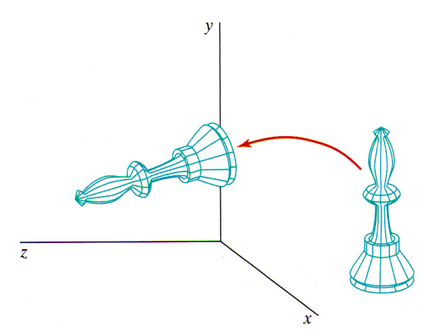
\includegraphics[width=0.7\textwidth]{Figures/rx}
			\caption{Rotação em torno do eixo $x$.}
			\end{center}
	\end{figure}
	
\end{frame}

%%%%%%%%%%%%%%%%%%%%%%%%%%%%%%%%%%%%%%%%%%%%%%%%%%%%%%%%%%%%%%%%%%%%%%%%%%%%%%%%%%%%%%%%%%
\begin{frame}
\frametitle{Rotação 3D}

	\begin{block}{Rotação 3D no eixo $y$}
		\begin{itemize}
			\item Levando em consideração a permutação citada, a rotação no eixo $y$ é composta da seguinte equação:\\
			\begin{eqnarray*}
				\begin{bmatrix}
					x' \\
					y' \\
					z' \\
					1
				\end{bmatrix} = 
				\begin{bmatrix}
					cos \theta	& sen \theta		& 0 & 0 \\
					0			& 1				& 0 & 0 \\
					-sen \theta	& cos \theta	& 0 & 0 \\
					0			& 0				& 0	& 1
				\end{bmatrix}
				\cdot \begin{bmatrix}
					x \\
					y \\
					z \\
					1
				\end{bmatrix}
			\end{eqnarray*}
		\end{itemize}
	\end{block}
	
\end{frame}

%%%%%%%%%%%%%%%%%%%%%%%%%%%%%%%%%%%%%%%%%%%%%%%%%%%%%%%%%%%%%%%%%%%%%%%%%%%%%%%%%%%%%%%%%%
\begin{frame}
\frametitle{Rotação 3D}


	\begin{figure}[!h]
			\begin{center}
			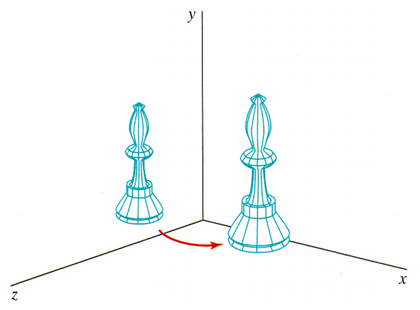
\includegraphics[width=0.7\textwidth]{Figures/ry}
			\caption{Rotação em torno do eixo $y$.}
			\end{center}
	\end{figure}
	
\end{frame}

%%%%%%%%%%%%%%%%%%%%%%%%%%%%%%%%%%%%%%%%%%%%%%%%%%%%%%%%%%%%%%%%%%%%%%%%%%%%%%%%%%%%%%%%%%
\begin{frame}
\frametitle{Rotação 3D}

	\begin{block}{Inversa da Rotação 3D}
		\begin{itemize}
			\item A inversa de uma rotação em $\theta$, é dada fazendo a rotação em $-\theta$.
			\item Como o que muda é apenas o sinal do seno, a inversa também pode ser obtida por $\textbf{R}^{-1} = \textbf{R}(-\theta)$.
		\end{itemize}
	\end{block}
	
\end{frame}


%%%%%%%%%%%%%%%%%%%%%%%%%%%%%%%%%%%%%%%%%%%%%%%%%%%%%%%%%%%%%%%%%%%%%%%%%%%%%%%%%%%%%%%%%%
\begin{frame}
\frametitle{Rotação Geral 3D}

	\begin{block}{Rotação Geral 3D}
		\begin{itemize}
			\item .
		\end{itemize}
	\end{block}
	
\end{frame}

%----------------------------------------------------------------------------------------

\end{document} 